
\section{Introduction}\label{intro}
% Introduce and motivate your project
Currently, no topic is hotter than machine learning and artificial intelligence. We are surrounded by it in our daily lives, from the ads we see on social media to the recommendations we get on Netflix. We focus on deep reinforcement learning (DRL), a subfield of machine learning. DRL employs deep neural networks to approximate the value function or policy function of a reinforcement learning (RL) agent, which circumvent the curse of dimensionality inherent to dynamic programming. DRL has been successfully applied to many domains, such as robotics, video games, and finance.\footnote{\url{https://github.com/AI4Finance-Foundation/FinRL-Meta}} For example, with the help of DRL, the program AlphaGo defeated the world champion in the game of Go \citep{silver_mastering_2016}.

However, despite the ongoing frenzy about these breakthroughs, applications of DRL in industrial contexts, such as inventory management, remain rather scarce. The true strength of these general learning algorithms is that they provide a way to solve a diversity of problems rather than relying on extensive domain knowledge or restrictive assumptions. In the inventory management literature, a variety of model-specific heuristics exists; it typically depends on the model assumptions which heuristic performs best. In contrast, DRL algorithms are easily accessible and can be applied to any sequential decision-making problem. As such, DRL could be perceived as a general purpose technology that can serve many different purposes.

In this project, we test the use of DRL in one classical inventory problems, namely the lost sales inventory problem. In this problem, a retailer faces stochastic demand and has to decide how much to order from a supplier since there is a positive holding cost each period. The customers walk away if the inventory is not enough to satisfy their demand and it incurs a goodwill lost to the retailer. The goal of the retailer is to maximize the expected total profit. Though it's a conceptually simple problem, little is known about the optimal policy structure since the traditional dynamic programming method quickly becomes intractable as the problem size grows, i.e., the leading time of the order increases.

\section{Related Work}
Discuss relevant prior studies and highlight their difference to your project
\citet{oroojlooyjadid_deep_2022} apply deep Q learning to the beer distribution game. The beer game consists of a serial supply chain network with four agents—a retailer, a warehouse, a distributor, and a manufacturer—that must make independent replenishment decisions with limited information. They show that when playing with teammates who follow a base-stock policy, our algorithm obtains nearoptimal order quantities. More important, it performs significantly better than a base-stock policy when other agents use a more realistic model of human ordering behavior.

\citet{gijsbrechts_can_2022} is another paper using DRL. The paper differs from \citet{oroojlooyjadid_deep_2022} in two distinctive ways. First, they provide optimality gaps on three different inventory problems whose stochastic dynamic program becomes quickly intractable. Second, they show the versatility of DRL by applying it to three different inventory problems with limited modification of the algorithm, thereby demonstrating that DRL resembles a general purpose technology.

This project is inspired by \citet{gijsbrechts_can_2022}. We use a simple DRL algorithm to solve the lost sales inventory problem.


\section{RL Environment}
% Introduce the environment and explain any changes you made or developed to the environment
Since there is no existing RL environment for the lost sales inventory problem, we develop our own environment. The environment is a discrete-time, finite-horizon, and finite-state Markov decision process (MDP). The state space is the inventory level, and the action space is the order quantity. The transition probability is the probability of demand. The reward function is the profit function defined in the next section. The agent is a standard deep Q network (DQN) with a fully connected neural network as the function approximator. The agent is trained with the Adam optimizer and the mean squared error loss function. We use experience replay and target network to stabilize the training process. In the following sections, we will discuss the details of the environment and the agent.

\section{Methodology}
% Describe technical details such as RL algorithm (and its parameters), action space, observation space, and reward function
\subsection{Environment}
\begin{table}[H]
    \centering
    \begin{tabular}{|l|l|}
        \hline
        \textbf{Parameter}             & \textbf{Value}      \\
        \hline
        \texttt{max\_warehouse\_level} & 20                  \\
        \texttt{max\_order}            & 15                  \\
        \texttt{max\_demand}           & 12                  \\
        \texttt{min\_demand}           & 8                   \\
        \texttt{state\_space}          & [0, 1, 2, ..., 20]  \\
        \texttt{action\_space}         & [0, 1, 2, ..., 15]  \\
        \texttt{demand\_space}         & [8, 9, 10, ..., 12] \\
        \texttt{price}                 & 10                  \\
        \texttt{wholesale\_price}      & 5                   \\
        \texttt{holding\_cost}         & 1                   \\
        \texttt{lost\_sale\_cost}      & 1                   \\
        \texttt{over\_order\_cost}     & 3                   \\
        % \texttt{transition\_function} & \textit{function reference} \\
        \hline
    \end{tabular}
    \caption{Parameters}
    \label{tab:pars}
\end{table}
We initilize the self-defined InventoryManagement environment using the parameters in \Cref{tab:pars}. For simplicity, we consider only discrete values for the state space, action space, and demand space. Also, the \textbf{max\_order} is set to control the quantity the retailer order each time. This is relavant since in reality, the retailer can only order a limited quantity relative to her inventory level each time for many reasons. The price, wholesale price, holding cost, lost sale cost, and over order cost can be changed to reflect different scenarios. In this case, we use \text{over\_order\_cost} to penalize the retailer for ordering too much.


For each step, we have the reward $r_t$ at time $t$ as
\begin{equation}
    r_t = p\min\{I_{t}, D_t\} - p_w a_t - p_l\left[D_t-I_t\right]^+ - p_h\left[I_t-D_t\right]^+,
\end{equation}
where $p$ is the retail price, $I_t$ is the state starting at $t$, i.e., the inventory level, $D_t$ is realized random demand at time $t$, $p_w a_t$ is the wholesale price for the order arriving at $t+1$, $a_t$ is the action which is the order quantity at time $t$ which has a lead time of $1$, $p_l$ is the cost of lost sales and $p_h$ is the holding cost.

Here, for the simplicity of our project, we restrict the state space to be 1-dimensional, i.e., the order with leading time 1. However, the environment can be easily extended to higher dimensions. For example, we can add the order with leading time 2, 3, etc. to the state space which might be more realistic. For example, considering a leading time of 2, the state space will be 2-dimensional, $(I_t,I_{t+1})$. The the retailer order $a_t$, then the state space at $t+1$ will be $(I_{t+1},[I_{t+1}-D_{t+1}]^++a_t)$. For each episode, we want to maximize the total reward
\begin{equation}
    \sum_{t=1}^T \gamma^t r_t
\end{equation}
where $T$ is the total number of steps in each episode and $\gamma$ is the discount factor which is set to $0.99$ in our project.



\subsection{Network Architecture}
Though it seems that multi-arm bandit can solve this problem, we still employ DQN since it can be easily generalized to higher dimendional state space.
\begin{verbatim}
class DQN(nn.Module):
    def __init__(self, state_space, action_space):
        super(DQN, self).__init__()
        self.action_space = action_space
        self.fc1 = nn.Linear(state_space, 64)
        self.fc2 = nn.Linear(64, 32)
        self.fc3 = nn.Linear(32, action_space)
    def forward(self, x):
        x = torch.relu(self.fc1(x))
        x = torch.relu(self.fc2(x))
        x = self.fc3(x)
        return x
\end{verbatim}

\begin{verbatim}
class Agent:
    def __init__(self, state_space, action_space):
        self.action_space = action_space 
        self.state_space = state_space
        self.epsilon = 1.0
        self.epsilon_min = 0.01
        self.epsilon_decay = 0.99
        self.gamma = 0.99
        self.batch_size = 2048
        self.memory = deque(maxlen=100000)
        self.model = DQN(state_space, action_space).to(device)
        self.optimizer = optim.Adam(self.model.parameters())
        self.MSE_loss = nn.MSELoss().to(device)
\end{verbatim}
We use a simple fully connected neural network as the function approximator. The memory is of length 100,000 and the batch size is 2048. The optimizer is Adam and the loss function is mean squared error. Also, we use a simple decaying epsilon greedy policy to balance exploration and exploitation.

Besides, we use experience replay and target network to stabilize the training process. The experience replay is implemented as follows. During the experience replay, we ramdomly sample a batch of data from the memory and update the network. Then we use the difference between the target network and the current network to update the target network by backpropagation.
\begin{verbatim}
def replay(self):
    if len(self.memory) < self.batch_size:
        return
    minibatch = random.sample(self.memory, self.batch_size)
    states, actions, rewards, next_states = map(np.array, zip(*minibatch))
    states = torch.tensor(states.reshape(-1, 1), 
                        dtype=torch.float32, device=device)
    next_states = torch.tensor(next_states.reshape(-1, 1), 
                        dtype=torch.float32, device=device)
    self.model.eval()
    next_state_values = self.model(next_states).detach().cpu().numpy()
    self.model.train()
    targets = rewards + self.gamma * (np.amax(next_state_values, axis=1)) 
    targets_full = self.model(states)
    targets_pred = targets_full.clone()
    targets_full[torch.arange(self.batch_size), torch.tensor(actions, device=device)]
     = torch.tensor(targets, dtype=torch.float32, device=device)

    loss = self.MSE_loss(targets_pred, targets_full)
    self.optimizer.zero_grad()
    loss.backward()
    self.optimizer.step()
\end{verbatim}

\subsection{Training}
After each step, we store the state, action, reward, and next state in the memory. Then if the memory is large enough, we sample a batch of data from the memory and update the network using the method mentioned in the previous subsection. 

\section{Experiments and Results}
% Report the experiment set-up and results
For this project, we set $T=1000$ and train the agent for 100 episodes. The training process is done on a personal PC with 12700K and RTX 4090. It takes about 10 minutes to train the agent for 100 episodes. 
\begin{figure}[H]
    \centering
    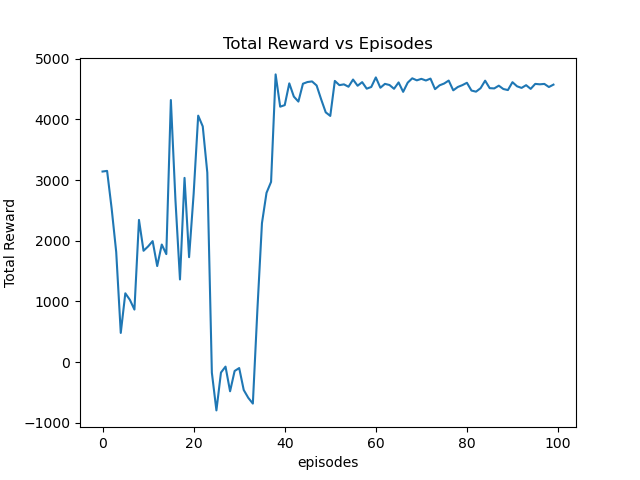
\includegraphics[width=0.8\textwidth]{figure/Total Reward vs Episodes copy.png}
    \caption{Total Reward during Training}
    \label{fig:total-reward}
\end{figure}
\Cref{fig:total-reward} shows the total reward during training. We can see that the total reward increases as the number of episodes increases which means the agent is learning. However, it suddenly decreses at epsiode 25. This is because the agent is exploring the environment and it might take some time to find the optimal policy. After that, the total reward increases again and reaches a plateau after episode 40. This is because the agent has found the optimal policy and it is just exploiting the environment. To make it clear, we plot the average order quantity during training in \Cref{fig:avg-order-quantity}. From the figure, we can see that the average order quantity is 14, i.e., near the maximum order quantity. But then it suddenly drops to around 0 to explore the environment. After that, it increases to around 10 which is the near-optimal order quantity since the distribution of demand is symmetric with mean 10.
\begin{figure}[H]
    \centering
    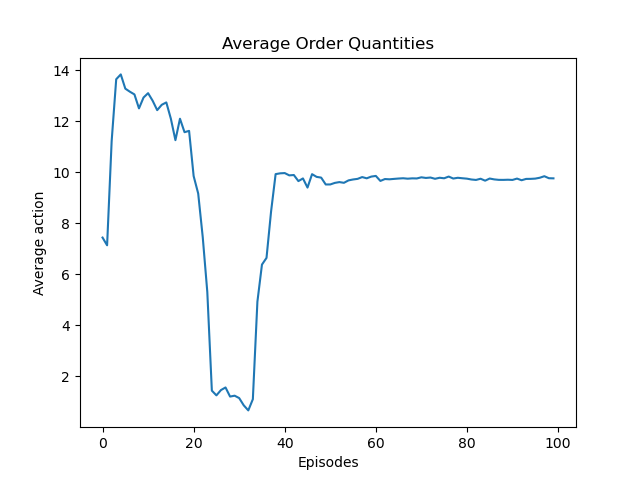
\includegraphics[width=0.8\textwidth]{figure/Average Order Quantities copy.png}
    \caption{Average Order Quantity during Training}
    \label{fig:avg-order-quantity}
\end{figure}

\subsection{Comparison with Base Order Policy}
Since we assume a leading time of 1, the traditional base-stock method is not feasible since it requires a leading time of 0 (the retailer need to order after the demand is realized). Thus, we compare our method to the base-order policy, i.e., the retailer always order the same amount at the start of each time period. We sample 1000 episodes for each policy and plot the histogram of the total reward in \Cref{fig:hist-base-9,fig:hist-base-10,fig:hist-base-11,fig:hist-base-12}. 

We can see that the best scenario for the base-stock policy in \Cref{fig:hist-base-10} can attain an average reward close to that in \Cref{fig:total-reward}. However, the average reward with DQN in \Cref{fig:total-reward} is around 4560 wich is larger than 4373 so that the DQN method performs better than the base-order policy in this case. This is intuitive since the base-order policy is a special case of the DQN method. The DQN method can find the optimal policy with respect to the current state (inventory level) while the base-order policy can only find the optimal policy in some special cases.

\begin{figure}[H]
    \centering
    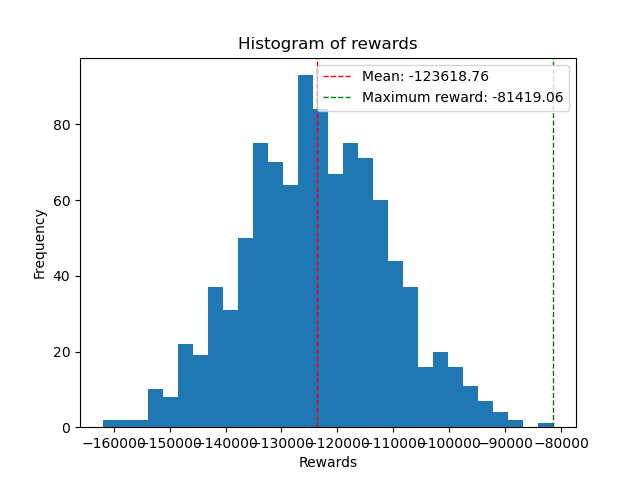
\includegraphics[width=0.8\textwidth]{figure/Histogram of rewards - Base 9.png}
    \caption{Histogram of Rewards for Base Order Policy with Base Order 9}
    \label{fig:hist-base-9}
\end{figure}
\begin{figure}[H]
    \centering
    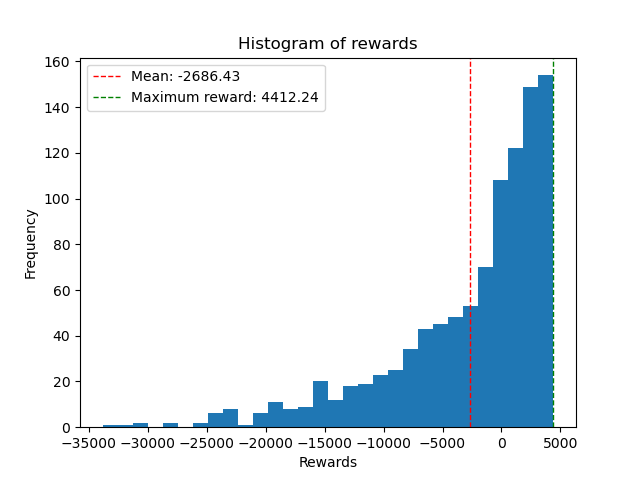
\includegraphics[width=0.8\textwidth]{figure/Histogram of rewards - Base 10.png}
    \caption{Histogram of Rewards for Base Order Policy with Base Order 10}
    \label{fig:hist-base-10}
\end{figure}
\begin{figure}[H]
    \centering
    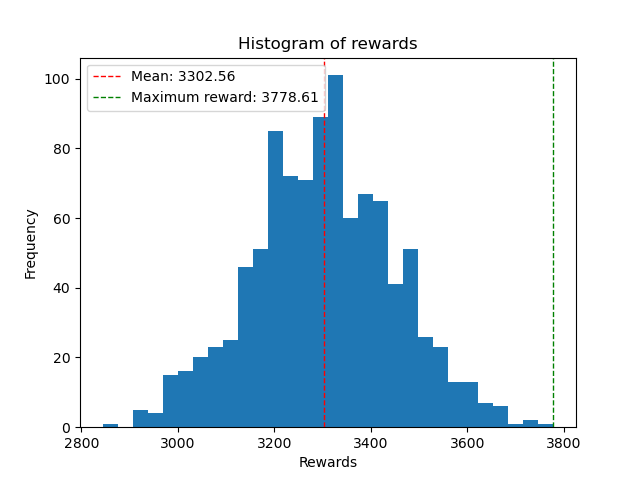
\includegraphics[width=0.8\textwidth]{figure/Histogram of rewards - Base 11.png}
    \caption{Histogram of Rewards for Base Order Policy with Base Order 11}
    \label{fig:hist-base-11}
\end{figure}
\begin{figure}[H]
    \centering
    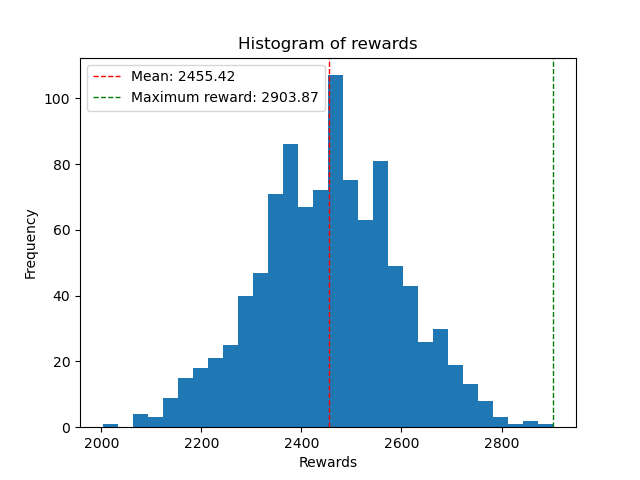
\includegraphics[width=0.8\textwidth]{figure/Histogram of rewards - Base 12.png}
    \caption{Histogram of Rewards for Base Order Policy with Base Order 12}
    \label{fig:hist-base-12}
\end{figure}


\section{Conclusion and Future Work}
% Summarize your project and discuss possible extensions of the project
In this project, we develop a RL environment for the lost sales inventory problem and apply DQN to solve it. We show that DQN can find the optimal policy for the lost sales inventory problem. Also, we compare our method with the base-order policy and show that our method is better than the base-order policy. 

But we only consider a simple DQN algorithm in this project. There are many other algorithms that can be applied to this problem. For example, we can use a more advanced algorithm such as double DQN or dueling DQN. Also, the training process can be improved. For example, we can use prioritized experience replay to improve the training process. Besides, we can also extend the environment to higher dimensions. For example, we can add the order with leading time 2, 3, etc. to the state space which might be more realistic. Currently, only 1d state space costs around 10 minutes to train for 100 episodes. If we add the order with leading time 2, 3, etc. to the state space, the training process will be much slower. Thus, we can use a more powerful computer or use a more efficient algorithm to speed up the training process. For example, use more advanced exploration methods such as noisy net or use a more efficient algorithm such as PPO.